\documentclass{article}

\usepackage{fancyhdr} % Required for custom headers
\usepackage{lastpage} % Required to determine the last page for the footer
\usepackage{extramarks} % Required for headers and footers
\usepackage[usenames,dvipsnames]{xcolor} % Required for custom colors
\usepackage{graphicx} % Required to insert images
\usepackage{listings} % Required for insertion of code
\usepackage{courier} % Required for the courier font
\usepackage{lipsum} % Used for inserting dummy 'Lorem ipsum' text into the template
\usepackage{hyperref}

\hypersetup{
    colorlinks=true,
    %linkbordercolor={white},
    %urlbordercolor={white},
    %runbordercolor={white},
    %citebordercolor={white},
    linkcolor={black},
    menucolor = {black},
    urlcolor = {blue},
    runcolor = {black},
    citecolor = {black},
    anchorcolor = {blue}
}

\topmargin=-0.45in
\evensidemargin=0in
\oddsidemargin=0in
\textwidth=6.5in
\textheight=9.0in
\headsep=0.25in

\linespread{1.1} % Line spacing

% Set up the header and footer
\pagestyle{fancy}
\lhead{\AssName} % Top left header
\rhead{\DocName} % Top right header
\lfoot{\DocRef} % Bottom left footer
\cfoot{email: team@apertus.org} % Bottom center footer
\rfoot{Page\ \thepage\ of\ \protect\pageref{LastPage}} % Bottom right footer
\renewcommand\headrulewidth{0.4pt} % Size of the header rule
\renewcommand\footrulewidth{0.4pt} % Size of the footer rule

\setlength\parindent{0pt} % Removes all indentation from paragraphs






%----------------------------------------------------------------------------------------
%	CODE CONFIGURATION
%----------------------------------------------------------------------------------------

\definecolor{MyDarkGreen}{rgb}{0.0,0.4,0.0} % This is the color used for comments
\lstloadlanguages{Perl} % Load Perl syntax for listings, for a list of other languages supported see: ftp://ftp.tex.ac.uk/tex-archive/macros/latex/contrib/listings/listings.pdf
\lstset{language=Perl, % Use Perl in this example
        frame=single, % Single frame around code
        basicstyle=\small\ttfamily, % Use small true type font
        keywordstyle=[1]\color{Blue}\bf, % Perl functions bold and blue
        keywordstyle=[2]\color{Purple}, % Perl function arguments purple
        keywordstyle=[3]\color{Blue}\underbar, % Custom functions underlined and blue
        identifierstyle=, % Nothing special about identifiers                                         
        commentstyle=\usefont{T1}{pcr}{m}{sl}\color{MyDarkGreen}\small, % Comments small dark green courier font
        stringstyle=\color{Purple}, % Strings are purple
        showstringspaces=false, % Don't put marks in string spaces
        tabsize=5, % 5 spaces per tab
        %
        % Put standard Perl functions not included in the default language here
        morekeywords={rand},
        %
        % Put Perl function parameters here
        morekeywords=[2]{on, off, interp},
        %
        % Put user defined functions here
        morekeywords=[3]{test},
       	%
        morecomment=[l][\color{Blue}]{...}, % Line continuation (...) like blue comment
        numbers=left, % Line numbers on left
        firstnumber=1, % Line numbers start with line 1
        numberstyle=\tiny\color{Blue}, % Line numbers are blue and small
        stepnumber=5 % Line numbers go in steps of 5
}

% Creates a new command to include a perl script, the first parameter is the filename of the script (without .pl), the second parameter is the caption
\newcommand{\perlscript}[2]{
\begin{itemize}
\item[]\lstinputlisting[caption=#2,label=#1]{#1.pl}
\end{itemize}
}


%----------------------------------------------------------------------------------------
%	STRUCTURE COMMANDS
%----------------------------------------------------------------------------------------

% Header and footer for when a page split occurs within a problem environment
\newcommand{\enterProblemHeader}[1]{
\nobreak\extramarks{#1}{#1 continued on next page\ldots}\nobreak
\nobreak\extramarks{#1 (continued)}{#1 continued on next page\ldots}\nobreak
}

% Header and footer for when a page split occurs between problem environments
\newcommand{\exitProblemHeader}[1]{
\nobreak\extramarks{#1 (continued)}{#1 continued on next page\ldots}\nobreak
\nobreak\extramarks{#1}{}\nobreak
}

\setcounter{secnumdepth}{5} % Makes sure that the indexing tree has 5 tiers
\setcounter{tocdepth}{5}

\newcommand{\homeworkProblemName}{}
\newenvironment{homeworkProblem}[1][Problem \arabic{homeworkProblemCounter}]{ % Makes a new environment called homeworkProblem which takes 1 argument (custom name) but the default is "Problem #"
\stepcounter{homeworkProblemCounter} % Increase counter for number of problems
\renewcommand{\homeworkProblemName}{#1} % Assign \homeworkProblemName the name of the problem
\section{\homeworkProblemName} % Make a section in the document with the custom problem count
\enterProblemHeader{\homeworkProblemName} % Header and footer within the environment
}{
\exitProblemHeader{\homeworkProblemName} % Header and footer after the environment
}

\newcommand{\problemAnswer}[1]{ % Defines the problem answer command with the content as the only argument
\noindent\framebox[\columnwidth][c]{\begin{minipage}{0.98\columnwidth}#1\end{minipage}} % Makes the box around the problem answer and puts the content inside
}

\newcommand{\homeworkSectionName}{}
\newenvironment{homeworkSection}[1]{ % New environment for sections within homework problems, takes 1 argument - the name of the section
\renewcommand{\homeworkSectionName}{#1} % Assign \homeworkSectionName to the name of the section from the environment argument
\subsection{\homeworkSectionName} % Make a subsection with the custom name of the subsection
\enterProblemHeader{\homeworkProblemName\ [\homeworkSectionName]} % Header and footer within the environment
}{
\enterProblemHeader{\homeworkProblemName} % Header and footer after the environment
}

\definecolor{keywordBack}{HTML}{FFEDED}
\newcommand{\importantKeyword}[1]{\colorbox{keywordBack}{\textcolor{BrickRed}{#1}}}

%----------------------------------------------------------------------------------------
%	NAMING
%----------------------------------------------------------------------------------------

\newcommand{\DocRef}{ABM.01.01.En.} % Foot Left
\newcommand{\AssName}{apertus° Association} % Head Left
\newcommand{\DocName}{AXIOM Beta User Manual} % Head Right

%----------------------------------------------------------------------------------------
%	TITLE PAGE
%----------------------------------------------------------------------------------------

\title{
\vspace{2in}
\textmd{\textbf{\hmwkClass:\ \hmwkTitle}}\\
\normalsize\vspace{0.1in}\small{Due\ on\ \hmwkDueDate}\\
\vspace{0.1in}\large{\textit{\hmwkClassInstructor\ \hmwkClassTime}}
\vspace{3in}
}

\author{\textbf{\hmwkAuthorName}}
\date{} % Insert date here if you want it to appear below your name

%----------------------------------------------------------------------------------------




\begin{document}

\begin{titlepage}
\begin{center}

\includegraphics[height=5cm]{images/Apertus_Logo_FullText}\\
\end{center}
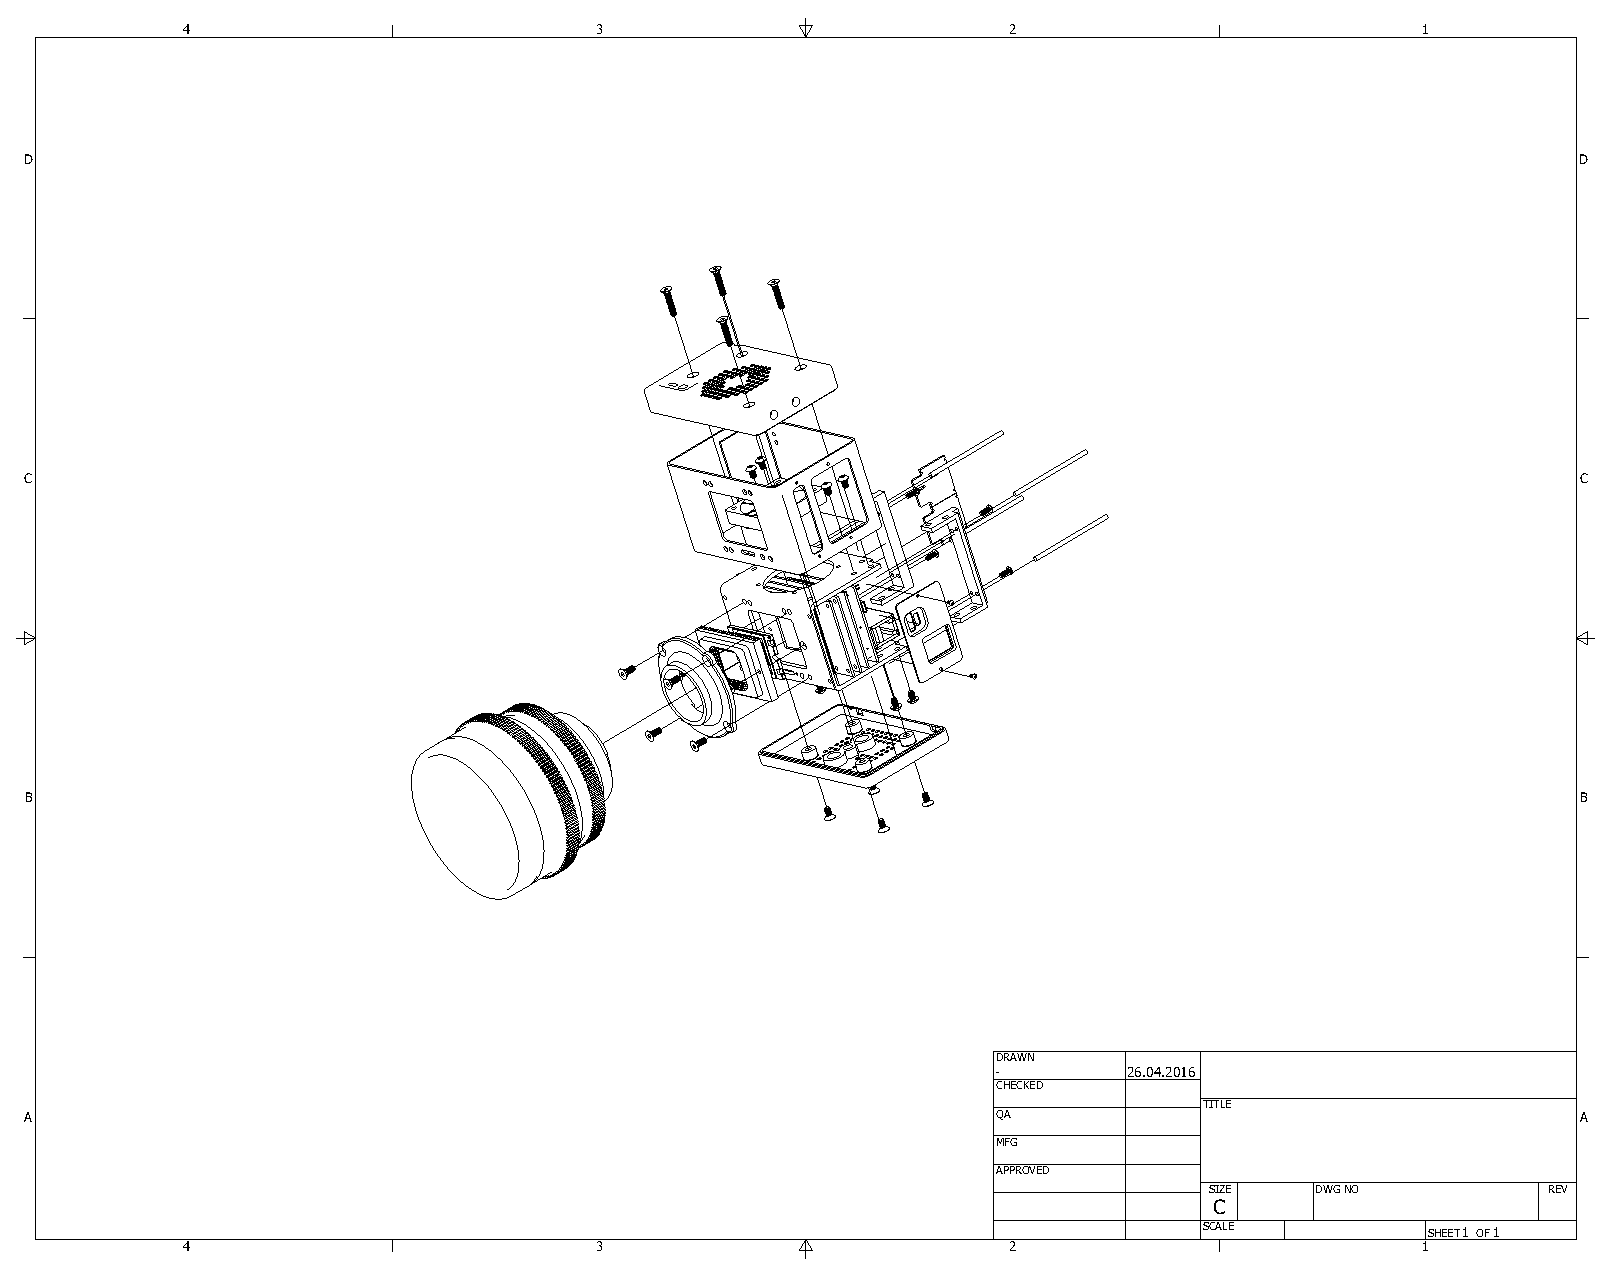
\includegraphics[height=13cm]{images/explosion-full}\\

\textbf{AXIOM Beta User Guide}\\

Permission is granted to copy, distribute and/or modify this document under the terms of the Creative Commons Attribution 4.0 International Public License (CC BY-SA 4.0).\\

Published by apertus° Association.\\


For more information, email team@apertus.org or visit \href{https://apertus.org}{apertus.org}

\end{titlepage}

\tableofcontents

\vspace*{\fill}
\textbf{Note:} In some instances the instructions we have prepared are written in a manor that can be followed by people without a deep technical knowledge. If you are an advanced user please keep this in mind.\\
\\This document has been compiled using LaTeX and its files are stored in the apertus GitHub repository here. If you choose to make any changes to this document please notify a member of the Team so that those changes can be implimented into instances of this guide that are being made available in other locations and formats eg. the project's Wiki page.

\newpage

\section{General Informaion}


\textbf{Notes on Userspace:} Arch Linux comes with systemd, which has one advantage that the boot process is incredibly fast. Standard tools such as sshd and dhcpcd have been preinstalled.\\

One idea to store camera relevant parameters inside the camera and provide access from most programming languages is to use a database like \href{http://en.wikipedia.org/wiki/Berkeley_DB}{http://en.wikipedia.org/wiki/Berkeley\_DB}


\subsection{AXIOM Beta Connector Overview}
	\subsection{Mountpoints}
	\subsection{Accessories and connected devices}
	

\section{Operating Basics}

\subsection{Prepare your AXIOM Beta for use}

Use a micro-USB cable to connect the camera's MicroZed development board (USB UART) to a computer. The MicroZed board is the backmost, red PCB. (There is another micro-USB socket on the Power Board, but that is the JTAG Interface.)\\

1. Connect the ethernet port on the MicroZed to an ethernet port on your computer. You might have to use an ethernet adapter on newer, smaller machines which come without a native ethernet port.\\ 

2. Connect the AC adapter to the camera's Power Board. (The power cord plugs into an adapter that connects to the Power Board; to power the camera off at a later point, you need not disconnect the adapter from the board but can just unplug the cord from the adapter.)


\subsection{Prepare your computer for use with AXIOM Beta}

\textbf{Overview -} To communicate with your AXIOM Beta camera, you will send it instructions via your computer's command line.\\

In case you have not worked with a shell (console, terminal) much or ever before, we have prepared detailed instructions to help you get you set up. The steps which need to 	be taken to prepare your machine sometimes differ between operating systems, so pick the ones that are applicable to you(r system). \\

Note that dollar signs placed in front of commands are not meant to be typed in but denote 	the command line prompt (a signal indicating the computer is ready for user input). It is used in documentation to differentiate between commands and output resulting from commands. The prompt might look different on your machine (e.g. an angled bracket >) and be preceded by your user name, computer name or the name of the directory which you are currently inside.



\subsubsection{USB to UART Drivers}

For the USB connection to work, you will need drivers for bridging USB to UART (USB to serial). (Under Linux this works out of the box in most 	distributions) for other operating systems they can be 

\hyperlink{https://www.silabs.com/products/development-tools/software/usb-to-uart-bridge-vcp-drivers}{downloaded}
downloaded from e.g. Silicon Labs' website – pick the software provided for your OS and install it. \\

\subsubsection{Serial Console}
\paragraph{Linux Setup}
\paragraph{MAC OSX Setup}
\paragraph{Minicom Configuration}
\subsubsection{Serial connection (via USB)}
\paragraph{Connect using Minicom}\mbox{}\\
Note that you will not be able to use the terminal window you initiate the serial connection in for anything else (it needs to remain open while you access the camera), so it might make sense to open a separate window just for this purpose.

With minicom installed and properly configured, all you need to do is run the following command to start it with the correct settings:

\begin{lstlisting}[language=bash,frame=none,xleftmargin=.25in,belowskip=2em, aboveskip=2em]
$ minicom -8 USB0
\end{lstlisting}

On successful connection, you will be prompted to enter user credentials (which are needed to log into the camera).

If your terminal remains blank except for the minicom welcome screen/information about your connection settings, try pressing enter. If this still does not result in the prompt for user credentials – while testing, we discovered the initial connection with minicom does not always work – disconnect the camera from the power adapter, then reconnect it: in your minicom window you should now see the camera's operating system booting up, followed by the login prompt. (From then on, connecting with minicom should work smoothly and at most require you to press enter to make the login prompt appear.)

\paragraph{Connect using Screen}
\paragraph{Disconnect}
\subsubsection{Ethernet connection (using SSH)}
\paragraph{SSH Keys how-to for Linux and Mac}
\subparagraph{Storage location/Find existing keys}
\subparagraph{SSH key creation}
\paragraph{Get or set IP address}
\paragraph{IP address check}
\paragraph{Set IP address}
\paragraph{Establish a connection via key}
\paragraph{Password-based authentication}
\subsubsection{Start the camera}
\subsubsection{WiFi access point setup}
\section{Writing Images}

For writing uncompressed full resolution full bitdepth raw images the AXIOM Beta uses a software called cmv_snap3.\\

It is located in the /root/ directory and writes the images data directly to STDOUT.\\

cmv_snap3 writes images in the \href{https://wiki.apertus.org/index.php/RAW12}{RAW12} format. Writing one image takes a few seconds depending on where the image is written to so this method is not viable for recording video footage other than timelapse. 




\subsection{Capture Still Images}
\subsubsection{Parameters}

The following parameters are available:

\begin{lstlisting}[language=bash,morekeywords=$,keywordstyle=\bfseries,frame=none,xleftmargin=.25in,belowskip=2em, aboveskip=2em]
    ./cmv_snap3 -h
    This is ./cmv_snap3 V1.10
    options are:
    -h        print this help message
    -8        output 8 bit per pixel
    -2        output 12 bit per pixel
    -d        dump buffer memory
    -b        enable black columns
    -p        prime buffer memory
    -r        dump sensor registers
    -t        enable cmv test pattern
    -z        produce no data output
    -e <exp>  exposure times
    -v <exp>  exposure voltages
    -s <num>  shift values by <num>
    -S <val>  writer byte strobe
    -R <fil>  load sensor registers
\end{lstlisting} 

\textbf{Examples}\\

Images can be written directly to the cameras internal micro SD card like this (10 milliseconds exposure time, 16bit):

\begin{lstlisting}[language=bash,morekeywords=$,keywordstyle=\bfseries,frame=none,xleftmargin=.25in,belowskip=2em, aboveskip=2em]
./cmv_snap3 -e 10ms > image.raw16
\end{lstlisting} 

Write image plus metadata (sensor configuration) to cameras internal micro SD card (20 milliseconds exposure time, 12bit): 

\begin{lstlisting}[language=bash,morekeywords=$,keywordstyle=\bfseries,frame=none,xleftmargin=.25in,belowskip=2em, aboveskip=2em]
./cmv_snap3 -2 -r -e 20ms > image.raw12
\end{lstlisting} 

You can also use cmv_snap3 to change to exposure time (to 5 milliseconds in this example) without actually capturing an image, for the that -z parameter is used to not produce any data output: 

\begin{lstlisting}[language=bash,morekeywords=$,keywordstyle=\bfseries,frame=none,xleftmargin=.25in,belowskip=2em, aboveskip=2em]
./cmv_snap3 -z -e 5ms
\end{lstlisting} 

That cmv_snap3 writes data to STDOUT makes it very versatile, we can for example capture images from and to a remote Linux machine connected to the Beta via Ethernet easily (lets assume the AXIOM Betas camera IP is set up as: 192.168.0.9 - SSH access has to be set up for this to work with a keypair) 

\begin{lstlisting}[language=bash,morekeywords=$,keywordstyle=\bfseries,frame=none,xleftmargin=.25in,belowskip=2em, aboveskip=2em]
ssh root@192.168.0.9 "./cmv_snap3 -2 -r -e 10ms" > snap.raw12
\end{lstlisting} 

To pipe the data into a file and display it at the same time with imagemagick on a remote machine: 

\begin{lstlisting}[language=bash,morekeywords=$,keywordstyle=\bfseries,frame=none,xleftmargin=.25in,belowskip=2em, aboveskip=2em]
    ssh root@192.168.0.9 "./cmv_snap3 -2 -r -e 10ms" | tee snap.raw12 | display -size 4096x3072 -depth 12 gray:-
\end{lstlisting} 

Use imagemagick to convert raw12 file into a color preview image: 

\begin{lstlisting}[language=bash,morekeywords=$,keywordstyle=\bfseries,frame=none,xleftmargin=.25in,belowskip=2em, aboveskip=2em]
cat test.raw12 | convert \( -size 4096x3072 -depth 12 gray:- \) \( -clone 0 -crop -1-1 \) \( -clone 0 -crop -1+0 \) \( -clone 0 -crop +0-1 \) -sample 2048x1536 \( -clone 2,3 -average \) -delete 2,3 -swap 0,1 +swap -combine test_color.png
\end{lstlisting} 


With raw2dng compiled inside the camera you can capture images directly to DNG, without saving the raw12: 


\begin{lstlisting}[language=bash,morekeywords=$,keywordstyle=\bfseries,frame=none,xleftmargin=.25in,belowskip=2em, aboveskip=2em]
./cmv_snap3 -2 -b -r -e 10ms | raw2dng snap.DNG
\end{lstlisting} 


\textbf{Note:} Supplying exposure time as parameter is required otherwise cmv_snap3 will not capture an image. The exposure time can be supplied in "s" (seconds), "ms" (milliseconds), "us" (microseconds) and "ns" (nanoseconds). Decimal values also work (eg. "15.5ms"). 


\subsection{Image Overlays}

This section covers the mimg version 1.8 (see \href{https://github.com/apertus-open-source-cinema/beta-software/tree/master/mimg}{GitHub repo}), not the previous 1.6. 

AXIOM Beta features a full HD framebuffer that can be altered from the Linux userspace and is automatically "mixed" with the real time video from the image sensor on HDMI outputs.\\

The overlay could also be used to draw live histograms/scopes/HUD or menus.\\

The overlay in more recent firmware revisions supports alpha channel transparency. \\


\subsubsection{Internals}


The raw memory image is saved the following way: <ch0/12bit><ch1/12bit><ch2/12bit><ch3/12bit><overlay/16bit> \\

This means that for every 4 sensels there is only one overlay pixel. Meaning, while the CMV12000 image sensor is 4Kx3K the overlay is Full HD (1080p). 


\subsubsection{Prepare Images}

Convert 24bit PNG (1920x1080 pixels) with transparency to AXIOM Beta raw format: 

\begin{lstlisting}[language=bash,morekeywords=$,keywordstyle=\bfseries,frame=none,xleftmargin=.25in,belowskip=2em, aboveskip=2em]
convert input.png rgba:output.rgb
\end{lstlisting}

\textbf{Note :} This image format is different from \href{https://wiki.apertus.org/index.php/RAW12}{RAW12}.


\subsubsection{mimg}

mimg is software running on the camera that's used to load/alter anything related to overlays or test images.\\

Source code is available on \href{https://github.com/apertus-open-source-cinema/beta-software/tree/master/mimg}{GitHub}.

\begin{lstlisting}[language=bash,morekeywords=$,keywordstyle=\bfseries,frame=none,xleftmargin=.25in,belowskip=2em, aboveskip=2em]
    This is ./mimg V1.8
    options are:
    -h        print this help message
    -a        load all buffers
    -o        load as overlay
    -O        load as color overlay
    -r        load raw data
    -w        use word sized data
    -D <val>  image color depth
    -W <val>  image width
    -H <val>  image height
    -P <val>  uniform pixel color
    -T <val>  load test pattern
    -B <val>  memory mapping base
    -S <val>  memory mapping size
    -A <val>  memory mapping address
\end{lstlisting} 

\textbf{Examples:}\\


Clear overlay: 

\begin{lstlisting}[language=bash,morekeywords=$,keywordstyle=\bfseries,frame=none,xleftmargin=.25in,belowskip=2em, aboveskip=2em]
./mimg -a -o -P 0
\end{lstlisting} 


Load monochrome overlay: 

\begin{lstlisting}[language=bash,morekeywords=$,keywordstyle=\bfseries,frame=none,xleftmargin=.25in,belowskip=2em, aboveskip=2em]
./mimg -o -a file.raw
\end{lstlisting} 


Load color overlay: 

\begin{lstlisting}[language=bash,morekeywords=$,keywordstyle=\bfseries,frame=none,xleftmargin=.25in,belowskip=2em, aboveskip=2em]
./mimg -O -a file.raw
\end{lstlisting} 


Enable overlay: 

\begin{lstlisting}[language=bash,morekeywords=$,keywordstyle=\bfseries,frame=none,xleftmargin=.25in,belowskip=2em, aboveskip=2em]
gen_reg 11 0x0104F000
\end{lstlisting} 


Disable overlay: 

\begin{lstlisting}[language=bash,morekeywords=$,keywordstyle=\bfseries,frame=none,xleftmargin=.25in,belowskip=2em, aboveskip=2em]
gen_reg 11 0x0004F000
\end{lstlisting} 


\textbf{Old overlays}:\\

Overlays for mimg 1.6 are not compatible anymore. You can use

\begin{lstlisting}[language=bash,morekeywords=$,keywordstyle=\bfseries,frame=none,xleftmargin=.25in,belowskip=2em, aboveskip=2em]
convert -size 1920x1080 -depth 6 rgba:overlay_04.rgb overlay_04.png
\end{lstlisting} 

... to convert them to PNG before continuing with the preparation above. 
\section{Changing Camera Parameters}

Some itro text required\\

\subsection{Setting CMV12000 sensor registers}

\textbf{cmv\_reg}

Get and Set CMV12000 image sensor registers (CMV12000 sports 128x16 Bit registers).\\

Details for the sensor datasheet are on GitHub under \href{https://github.com/apertus-open-source-cinema/beta-hardware/tree/master/Datasheets}{Datasheets}\\

\textbf{Examples:}\\

Read register 115 (which contains the analog gain settings): 

\begin{lstlisting}[language=bash,morekeywords=$,keywordstyle=\bfseries,frame=none,xleftmargin=.25in,belowskip=2em, aboveskip=2em]
cmv_reg 115
\end{lstlisting} 

Return value:

\begin{lstlisting}[language=bash,morekeywords=$,keywordstyle=\bfseries,frame=none,xleftmargin=.25in,belowskip=2em, aboveskip=2em]
0x00
\end{lstlisting} 

Means we are currently operating at analog gain x1 = unity gain\\


Set register 115 to gain x2: 

\begin{lstlisting}[language=bash,morekeywords=$,keywordstyle=\bfseries,frame=none,xleftmargin=.25in,belowskip=2em, aboveskip=2em]
cmv_reg 115 1
\end{lstlisting}



\subsection{Setting Exposure Time}

To set the exposure time use the cmv\_snap3 tool with -z parameter (this will tell the software to not save the image): 

\begin{lstlisting}[language=bash,morekeywords=$,keywordstyle=\bfseries,frame=none,xleftmargin=.25in,belowskip=2em, aboveskip=2em]
./cmv_snap3 -e 9.2ms -z
\end{lstlisting}

\textbf{Note:} The exposure time can be supplied in "s" (seconds), "ms" (milliseconds), "us" (microseconds) and "ns" (nanoseconds). Decimal values also work (eg. "15.5ms"). 



\subsection{Setting gain value}

\textbf{set\_gain.sh}\\

Set gain and related settings (ADC range and offsets). 

\begin{lstlisting}[language=bash,morekeywords=$,keywordstyle=\bfseries,frame=none,xleftmargin=.25in,belowskip=2em]
    ./set_gain.sh 1 
    ./set_gain.sh 2
    ./set_gain.sh 3/3 # almost the same as gain 1
    ./set_gain.sh 3
    ./set_gain.sh 4
\end{lstlisting}



\subsection{Setting Gamma Values}

\textbf{gamma\_conf.sh}\\

Set the gamma value: 

\begin{lstlisting}[language=bash,morekeywords=$,keywordstyle=\bfseries,frame=none,xleftmargin=.25in,belowskip=2em]
    ./gamma_conf.sh 0.4
    ./gamma_conf.sh 0.9
    ./gamma_conf.sh 1
    ./gamma_conf.sh 2
\end{lstlisting}




\section{Image metadata}
\subsection{cmv hist}

\section{Output}
\subsection{HDMI}
\subsubsection{External HDMI Recording}
\subsubsection{Experimental UHD Raw Recording}
\subsubsection{EDL Parser}
\subsubsection{cmv perf3}
\subsection{SDI}
\subsection{Modes}
\subsection{Generator and HDMI Output}
\subsection{Stopping and Starting HDMI Live-stream}

\section{Processing}
\subsection{Image Acquisition Pipeline}
\subsection{HDMI Image Processing/Output Pipeline}
\subsection{SDI Image Processing/Output Pipeline}
\subsection{Image Processing Nodes}

\section{Converting}
\subsection{RAW12 to PGM}
\subsection{RAW12 to DNG}

\section{Maintenance}
\subsection{Firmware Backup}
\subsection{Firmware Restore}
\subsection{Image Sensor cleaning}

\section{Installations}
\subsection{Installing a webserver}
\subsection{Configuring a webserver}
\subsection{Installing AXIOM Beta Web GUI software}

\section{Colour Science}
\subsection{Black Calibration}
\subsection{Pattern Noise}
\subsection{Matrix Color Conversion} %See also mat4_conf.sh
\subsection{CMV12000 PLR}
\subsection{CMV12000 Response Curves}

\section{Associated Use-cases}
\subsection{Configuration for Photography}

\section{Hardware}
\subsection{PCB Stack Layout}
\subsubsection{Shields}
\subsubsection{Plugin Modules}
\subsubsection{EEPROM}
\subsection{PCB Revision Links}
\subsection{Power Supply}
\subsubsection{AC Power Supply}
\subsubsection{DC Power Supply}
\subsubsection{Active Battery Mount}
\subsection{Enclosure}
\subsubsection{Skeleton}
\subsubsection{Simple Enclosure}
\subsubsection{Transparent Acrylic Enclosure}
\subsection{Optical Information}
\subsubsection{Lens Mount}
\subsubsection{Lens Mount Overviews}
\subsubsection{Infra Red / Ultra Violet Cut-off Filter}
\subsubsection{Optical Low-pass Filter (OLPF)}

\section{Support}
\subsection{Contact Details and Communication Channels}
\subsection{Regional Communities}
\subsection{Useful Links}



%\\Test


\begin{lstlisting}[breaklines=true, breakatwhitespace=true]
    1: lo: <LOOPBACK,UP,LOWER_UP> mtu 65536 qdisc noqueue state UNKNOWN group default 
        link/loopback 00:00:00:00:00:00 brd 00:00:00:00:00:00
        inet 127.0.0.1/8 scope host lo
           valid_lft forever preferred_lft forever
        inet6 ::1/128 scope host 
           valid_lft forever preferred_lft forever
    2: eth0: <BROADCAST,MULTICAST,UP,LOWER_UP> mtu 1500 qdisc pfifo_fast state UP group default qlen 1000
        link/ether 00:0a:35:00:01:26 brd ff:ff:ff:ff:ff:ff
        inet 192.168.0.9/24 brd 192.168.0.255 scope global dynamic eth0
           valid_lft 172739sec preferred_lft 172739sec
        inet6 fe80::20a:35ff:fe00:126/64 scope link 
           valid_lft forever preferred_lft forever
\end{lstlisting}


\begin{lstlisting}
    cd ~/.ssh/
    cp authorized_keys authorized_keys.orig
\end{lstlisting}


ghgffghfg

\end{document}
